% ======================================================================
%  ICAIF '26 submission
%  Learned z-score forecasting for cross-exchange cryptocurrency spreads
%
%  Build:  tectonic gradient-boosting-cross-market-spread-prediction.tex
%
%  REVIEW (double-blind) build is the default:
%      \documentclass[sigconf,anonymous,review]{acmart}
%  CAMERA-READY: switch to \documentclass[sigconf]{acmart}, set
%  \anonsubmissionfalse below, and fill in the ACM rights-form commands.
% ======================================================================
\documentclass[sigconf,anonymous,review]{acmart}

%%% ----- Packages -----
\usepackage{booktabs}
\usepackage{amsmath}
\usepackage{multirow}
\usepackage{graphicx}
\usepackage{subcaption}

%%% ----- Anonymity toggle -----
% Must be kept in sync with the `anonymous' documentclass option: the class
% suppresses the author block automatically, but it cannot anonymise
% identifying URLs inside the body text.
\newif\ifanonsubmission
\anonsubmissiontrue

\newcommand{\datasetref}{%
  \ifanonsubmission
    the public dataset release (URL withheld for double-blind review)%
  \else
    \url{https://huggingface.co/datasets/SFU-fintech-AI/statarb-crypto-research}%
  \fi
}

\newcommand{\coderef}{%
  \ifanonsubmission
    the code repository (URL withheld for double-blind review)%
  \else
    \url{https://github.com/kevinl03/stochastic-spread-modeling}%
  \fi
}

%%% ----- ACM metadata -----
\setcopyright{none}
\acmConference[ICAIF '26]{7th ACM International Conference on AI in Finance}{November 14--17, 2026}{Milan, Italy}

\begin{document}

\title{Learned Z-Score Forecasting for Cross-Exchange Cryptocurrency
Spreads:\\A Gradient-Boosting Approach on Live Microstructure Data}

\author{Kevin Litvin}
\affiliation{%
  \institution{Simon Fraser University}
  \city{Burnaby}
  \state{British Columbia}
  \country{Canada}
}
\email{ktl13@sfu.ca}

\author{Tania Pocrnjic}
\affiliation{%
  \institution{Simon Fraser University}
  \city{Burnaby}
  \state{British Columbia}
  \country{Canada}
}
\email{tania_pocrnjic@sfu.ca}

\author{Ke Li}
\affiliation{%
  \institution{Simon Fraser University}
  \city{Burnaby}
  \state{British Columbia}
  \country{Canada}
}
\email{keli@sfu.ca}

% ======================================================================
%  ABSTRACT
% ======================================================================
\begin{abstract}
Cross-exchange price spreads for identical cryptocurrency assets are widely documented, yet the literature universally relies on rule-based z-score thresholds to generate trading signals. We demonstrate that a gradient-boosting model (LightGBM) can predict the next-snapshot z-score of same-asset cross-exchange spreads from live centralized-exchange data, replacing mechanical threshold rules with a learned forecast. The model ingests 68 features spanning lagged spread dynamics, orderbook imbalance, trade flow, funding rates, open interest, and cross-venue dispersion across 23 volatile assets and 6 exchanges at approximately one-minute granularity. A feature-group ablation shows that predictive power is concentrated in the lagged z-score trajectory and venue-pair identity; microstructure inputs do not improve filtered R$^2$ under this tree-ensemble protocol. The live-collected orderbook and trade-flow panel nonetheless cannot be reconstructed from historical exchange APIs, and we release it as a standalone dataset contribution for future architectures. A confidence filter trades only when the predicted z-score magnitude exceeds 0.5, selecting high-quality entries from the forecast distribution. In an 8-hour live paper-trading campaign, the filtered policy achieves directional accuracy of 76.9\%, prediction R$^2$ of 0.35, and an hourly portfolio Sharpe ratio of 2.41, with positive risk-adjusted returns in every observed hour. Under matched capacity constraints, the learned policy improves per-trade directional accuracy by 7.6 percentage points and mean profit by 71\% over a mechanical persistence baseline on identical settlement rules. These results establish that supervised z-score forecasting---dominated by recent spread trajectory---offers a strictly stronger trading signal than the mechanical z-score threshold rules that underpin existing high-frequency cryptocurrency pairs-trading systems.
\end{abstract}


%%% CCS concepts --- the CCSXML block and the \ccsdesc lines below are
%%% generated together by https://dl.acm.org/ccs/ccs.cfm and must match.
\begin{CCSXML}
<ccs2012>
  <concept>
    <concept_id>10010147.10010257.10010258.10010259.10010263</concept_id>
    <concept_desc>Computing methodologies~Supervised learning by regression</concept_desc>
    <concept_significance>500</concept_significance>
  </concept>
  <concept>
    <concept_id>10010405.10010455.10010461</concept_id>
    <concept_desc>Applied computing~Economics</concept_desc>
    <concept_significance>300</concept_significance>
  </concept>
  <concept>
    <concept_id>10002951.10003227.10003351</concept_id>
    <concept_desc>Information systems~Data mining</concept_desc>
    <concept_significance>300</concept_significance>
  </concept>
</ccs2012>
\end{CCSXML}

\ccsdesc[500]{Computing methodologies~Supervised learning by regression}
\ccsdesc[300]{Applied computing~Economics}
\ccsdesc[300]{Information systems~Data mining}

\keywords{statistical arbitrage, cryptocurrency, cross-exchange spreads,
gradient boosting, market microstructure, limit order book, live evaluation}

\maketitle

% ======================================================================
%  INTRODUCTION
% ======================================================================
\section{Introduction}\label{sec:intro}

Cryptocurrency markets are fragmented across dozens of centralized exchanges (CEXs), each with independent order books, heterogeneous fees, liquidity, and matching-engine latencies. Unlike equities, there is no consolidated tape that forces immediate price convergence. The result is recurrent cross-exchange price dislocations for \emph{identical} assets~\cite{makarov2020trading}---economically meaningful opportunities for same-asset statistical arbitrage, especially among high-volatility coins where short-lived Law-of-One-Price deviations appear at approximately one-minute granularity.

% ======================================================================
%  RELATED WORK
% ======================================================================
\section{Related Work}\label{sec:related}

We organize related work along two axes: (1)~the signal generation method (rule-based z-score thresholds vs learned models) and (2)~the market structure (single-exchange different-asset pairs vs cross-exchange same-asset spreads). Our work occupies the intersection of \emph{learned spread forecasting} and \emph{cross-exchange same-asset trading} with \emph{minute-scale microstructure features}, a combination that, to the best of our knowledge, no prior study addresses.

\subsection{Rule-Based Z-Score Pairs Trading in Crypto}

All existing crypto pairs-trading studies use rolling z-score thresholds or cointegration-derived signals at 1--5 minute frequencies on single exchanges, trading \emph{different} assets whose co-movement may break down as fundamentals diverge~\cite{fil2020pairs, tadi2021evaluation, ko2023pairs, tadi2025copula, palazzi2025trading}. Our work differs in three structural ways: we trade the \emph{same} asset across \emph{different} exchanges (where the Law of One Price guarantees mean-reversion), we train a model to \emph{predict the future z-score} rather than using it as a mechanical threshold signal, and we incorporate L2~orderbook, trade flow, and funding rate features that cannot be backfilled from exchange APIs.

\subsection{ML Models for Spread Prediction}

A smaller body of work trains models to predict spread dynamics. Tsoku and Makatjane~\cite{tsoku2026dl} train a DNN+LSTM ensemble to forecast spread dynamics on cointegrated cryptocurrency pairs but operate at lower frequency, on a single exchange, without microstructure features. Fischer et al.~\cite{fischer2019statistical} train a random forest on minute-binned lagged returns of 40~crypto coins, finding that alpha falls from 20.5~bps to 3.8~bps under a one-minute execution delay---a decay profile that makes execution latency a first-order threat to validity at our collector cadence (Section~\ref{sec:limitations}). Liou et al.~\cite{liou2024hft} use LOB features for spread prediction in equities pairs trading, paralleling our orderbook imbalance inputs but on a single exchange. Han and Li~\cite{han2024lstm} use LSTM as a trade filter on CSI~300 futures, a framing analogous to our confidence threshold ($|\hat{z}| \geq 0.5$).

\subsection{ML-Enhanced Pairs Trading on Equities}

Several equity-market papers establish the dual-metric reporting norms we follow. Sarmento et al.~\cite{sarmento2024ml} find that model abstention improves profit-per-trade on 1-minute Brazilian stock ratios, paralleling our confidence filter. Shen et al.~\cite{shen2022arbitrage} achieve R$^2$ of 92\% on CSI~300 spot-futures spreads with LSTM, though the high R$^2$ reflects slow-moving equity index spreads; our noisy crypto spreads yield R$^2$ of 0.35 on filtered entries. Perrone et al.~\cite{perrone2026pairs} reformulate statistical arbitrage as a panel-level prediction task on daily equity data. These studies operate at lower frequencies, on single exchanges, and without non-backfillable microstructure features.

\subsection{Positioning Summary}

Table~\ref{tab:positioning} summarizes the key dimensions along which our work differs from the closest related papers.

\begin{table}[h]
\caption{Positioning of this work relative to closest related papers. Columns indicate whether each study uses a learned model (vs rule-based), operates cross-exchange (vs single-venue), uses L2 orderbook or microstructure features, evaluates on live (non-backtest) data, and reports both forecast and trading metrics.}
\label{tab:positioning}
\small
\begin{tabular}{lccccc}
\toprule
\textbf{Paper} & \textbf{Learned} & \textbf{Cross-} & \textbf{L2/} & \textbf{Live} & \textbf{Dual} \\
 & \textbf{model} & \textbf{exch.} & \textbf{micro.} & \textbf{eval} & \textbf{metrics} \\
\midrule
Fil \& Kristoufek      & \texttimes & \texttimes & \texttimes & \texttimes & \texttimes \\
Tadi \& Kortchemski     & \texttimes & \texttimes & \texttimes & \texttimes & partial \\
Ko et al.               & \texttimes & \texttimes & \texttimes & \texttimes & \checkmark \\
Tadi \& Witzany         & \texttimes & \texttimes & \texttimes & \texttimes & \checkmark \\
Fischer et al.          & \checkmark & \texttimes & \texttimes & \texttimes & partial \\
Tsoku \& Makatjane      & \checkmark & \texttimes & \texttimes & \texttimes & partial \\
Liou et al.             & \checkmark & \texttimes & \checkmark & \texttimes & partial \\
Han \& Li               & \checkmark & \texttimes & \texttimes & \texttimes & \texttimes \\
\midrule
\textbf{This work}      & \checkmark & \checkmark & \checkmark & \checkmark & \checkmark \\
\bottomrule
\end{tabular}
\end{table}

No prior study combines all five properties. The closest papers in individual dimensions are Tsoku and Makatjane~\cite{tsoku2026dl} (learned crypto spread forecast, but lower frequency and single exchange), Liou et al.~\cite{liou2024hft} (LOB features for spread prediction, but equities and single exchange), and Fischer et al.~\cite{fischer2019statistical} (minute-scale ML on crypto, but cross-sectional rank prediction rather than pairwise spread forecasting). Our contribution is at the intersection: a learned z-score forecast on cross-exchange same-asset spreads, trained on non-backfillable minute-scale microstructure features, validated live with dual forecast and trading metrics.

% ======================================================================
%  METHODOLOGY
% ======================================================================
\section{Methodology}\label{sec:method}

\subsection{Cross-Exchange Spread and Z-Score Target}

Let $P_i^c(t)$ denote the mid-price of asset $c$ on exchange $i$ at snapshot $t$. For an exchange pair $(i, j)$, the cross-exchange spread in basis points is:
\begin{equation}
    S_{ij}^c(t) = \frac{P_i^c(t) - P_j^c(t)}{P_i^c(t)} \times 10{,}000
\end{equation}

Unlike traditional pairs trading where the spread between different assets may diverge permanently as fundamentals change, the cross-exchange spread for the same asset is anchored by the Law of One Price: absent frictions, $S_{ij}^c(t) \to 0$. In practice, fees, withdrawal delays, and matching-engine latency allow temporary price deviations for the same coin across different exchanges.

We normalize the spread into a rolling z-score:
\begin{equation}
    z_t = \frac{S_t - \hat{\mu}_w}{\hat{\sigma}_w}
\end{equation}
where $\hat{\mu}_w$ and $\hat{\sigma}_w$ are the estimated rolling mean and standard deviation over a window of $w$ snapshots, with a minimum period requirement before the z-score is defined. Model outputs $\hat{z}$ are therefore in units of this trailing $\hat{\sigma}_w$: $|\hat{z}|=1$ is a one-$\sigma$ forecasted dislocation. We use $w=300$ ($\text{MIN\_PERIODS}=90$); larger $w$ adds context but lengthens warmup (Section~\ref{sec:ablation}).

\subsection{Supervised Prediction Target}

The model's target is the \emph{future} z-score at horizon $H$:
\begin{equation}
    y_t = z_{t+H}
\end{equation}
computed via $\texttt{groupby(coin, pair).zscore.shift(-H)}$ on the training panel. This is a regression target, not a binary classification. The model predicts both the direction and magnitude of the z-score $H$ snapshots ahead, enabling a confidence filter on $|\hat{z}|$.

For the prediction model used in the paper-trading campaigns, $H = 1$ (predict the next snapshot's z-score), $w = 300$ snapshots, and $\text{MIN\_PERIODS} = 90$. Window length and confidence cutoff ($\tau$) selection is described in Section~\ref{sec:ablation}.

\subsection{Feature Engineering}\label{sec:features}

The model uses a 68-dimensional feature matrix per (coin, exchange-pair, snapshot), built from four synchronized live signal families: (i)~lagged cross-exchange spreads and rolling z-scores, with short momentum and acceleration of those series; (ii)~ticker top-of-book mids, bid--ask widths, and volumes; (iii)~L2 orderbook imbalance over the top~20 levels on each venue,
\begin{equation}
    \texttt{imbalance}_i = \frac{V_{\text{bid},i} - V_{\text{ask},i}}{V_{\text{bid},i} + V_{\text{ask},i}},
\end{equation}
with short lags of that ratio; and (iv)~recent trade-flow intensity and buy/sell imbalance, plus cross-venue aggregates (mid dispersion, BA/OB variability, and price ranks). $\texttt{coin}$ and $\texttt{pair}$ enter as LightGBM native categoricals so one panel model can specialize by asset and venue pair. Exact column names and construction details ship with the public dataset release (\datasetref); Section~\ref{sec:ablation} ablates the engineered spread/$z$ trajectory against raw live columns.

\subsection{Model: LightGBM Gradient Boosting}\label{sec:lgbm}

We train a single LightGBM~\cite{ke2017lightgbm} regression model on the pooled panel of all (coin, exchange-pair, snapshot) observations. The objective is squared error minimization on $y_t = z_{t+H}$.

We deliberately choose tree ensembles over the DNN/LSTM architectures common in prior spread-forecasting work: the feature matrix is a heterogeneous tabular panel (lags, microstructure, and native categoricals) for which tree models are a strong default inductive bias. As a classical Random Forest baseline on the same train/test feature matrix, we also fit a Random Forest regressor~\cite{breiman2001random} (regularized leaf size analogous to LightGBM's minimum child samples). LightGBM is the model used for validation-campaign evaluation; the Random Forest control is scored on the test set (Section~\ref{sec:results}).

\subsection{Trading Policy}\label{sec:policy}

At each live snapshot, the model generates a prediction $\hat{z}_{t+1}$ for every (coin, exchange-pair) observation. The trading policy is:

\begin{enumerate}
    \item Entry: open a position if $|\hat{z}_{t+1}| \geq \tau$ and the (coin, pair) slot is not already occupied. The paper protocol uses $\tau{=}0.9$.
    \item Direction: $\text{sign}(\hat{z}_{t+1})$. The model predicts the sign of the spread z-score at $t+1$ and bets accordingly.
    \item Capacity: at most $\text{max\_open} = 50$ positions open simultaneously, enforced by a first-come queue.
    \item Settlement: each position settles at $t+H$ (with $H=1$). The proxy profit is $\text{pnl\_proxy} = \text{direction} \times z_{t+H}$.
\end{enumerate}

The settlement proxy measures whether the z-score moved in the predicted direction and by how much, in z-score units. It is not a dollar profit metric and does not account for transaction fees or slippage.


\subsection{Evaluation Metrics}

We report both forecast quality and trading performance metrics:

\begin{itemize}
    \item \textbf{R$^2$}: fraction of variance in the realized $z_{t+H}$ explained by the model's predictions.
    \item \textbf{Directional accuracy (DirAcc)}: fraction of predictions where $\text{sign}(\hat{z}) = \text{sign}(z_{t+H})$.
    \item \textbf{Mean pnl\_proxy}: average $\text{direction} \times z_{t+H}$ across settled trades.
    \item \textbf{Per-trade Sharpe}: $\text{mean}(\text{pnl\_proxy}) / \text{std}(\text{pnl\_proxy})$ on the filtered trade set (Rf~$=0$), used to select $\tau$ in Section~\ref{sec:ablation}.
    \item \textbf{Hourly portfolio Sharpe ratio}: $\text{mean}(\Delta\text{equity}_h) / \text{std}(\Delta\text{equity}_h)$ where hourly equity includes realized closed-trade profits plus mark-to-market valuation of open positions as $\text{direction} \times z_t$. Risk-free rate is zero because the z-unit proxy has no currency denomination and represents forecast quality rather than economic returns.
\end{itemize}

All metrics are computed with a matched \textbf{naive persistence baseline} ($\hat{z}_{t+H} \leftarrow z_t$) scored on the identical row set.

% ======================================================================
%  EXPERIMENTAL SETUP
% ======================================================================
\section{Experimental Setup}\label{sec:setup}

\subsection{Data Collection}

We collect live microstructure data from centralized cryptocurrency exchanges using a custom collector that polls 9~signal families (orderbook, trades, ticker, funding, open interest, withdrawal status, exchange status, spread matrices, OHLCV) via REST API at approximately 60-second target cadence across 23~assets and 6~exchanges (Binance, Bybit, OKX, Coinbase, Kraken, MEXC). Under full signal load, the observed cadence is approximately 110~seconds per snapshot. Data collection protocol and signal schema are documented in the repository accompanying \datasetref.

\subsection{Train/Test Split}

All collection windows before July~25, 2026 form the training set; July~25--28 forms the held-out test set. The split is strictly chronological with no shuffling. The training set contains approximately 2.9~million (coin, exchange-pair, snapshot) feature rows spanning multiple collection windows from June--July 2026. Cross-sectional rows within a snapshot are structurally dependent (they share the same market state), so this row count should not be interpreted as independent samples.

\subsection{Live Paper-Trading Protocol}

For live validation, we run independent paper-trading campaigns that process incoming collector data in real time with no access to future snapshots. Capacity is $\text{max\_open} = 50$. The paper confidence gate is $\tau{=}0.9$ (Section~\ref{sec:ablation}).

\subsubsection{Campaign A: Jul~31 - TO REMOVE}

\begin{itemize}
    \item \textbf{Model}: 68-feature prediction model (\texttt{statarb\_lgbm.txt}).
    \item \textbf{Horizon}: $H = 1$ (predict next snapshot).
    \item \textbf{Z-score window}: 300~snapshots.
    \item \textbf{Duration}: approximately 8~hours of useful data (collector ran for 264~snapshots).
    \item \textbf{Warmup}: predictions become active after $\text{MIN\_PERIODS} = 90$ snapshots (approximately 2.5--3~hours).
    \item \textbf{Predictions scored}: 58,995 total; 2,026 rows with $|\hat{z}|\geq 0.9$.
\end{itemize}

We validate reuslts on a 72\-hour live trading campaign, using the same model and model parameters as in training and testing. 

\subsubsection{Campaign B: Aug~4--7 (\textasciitilde72h)}

\begin{itemize}
    \item \textbf{Model}: same 68-feature, $H{=}1$, $w{=}300$ policy as Campaign~A.
    \item \textbf{Duration}: $\approx$72.9~hours of active trading (50,690 closed trades; 1.01M scored predictions).
    \item \textbf{Role}: multi-day live stress test; primary $\tau{=}0.9$ metrics are the post-hoc paper-protocol subset of this book (Section~\ref{sec:ablation}).
\end{itemize}

\subsection{Baseline Definitions - NEED TO UPDATE }

\subsubsection{Naive persistence}

On every row where the model generates a prediction, we also record the naive forecast $\hat{z}_{t+H} \leftarrow z_t$ (the current z-score predicts the future z-score unchanged). R$^2$ and directional accuracy are computed for both model and naive on the \emph{identical} rows, ensuring that any performance difference is attributable to the model rather than to row selection.

\subsubsection{Mechanical z-score baselines}

We replay two mechanical trading rules on the Jul~31 signal panel under the same capacity constraints ($\text{max\_open} = 50$), settlement proxy, and paper gate $\tau{=}0.9$ as the model:

\begin{itemize}
    \item \textbf{Persistence}: enter when $|z_t| \geq 0.9$, direction $= \text{sign}(z_t)$.
    \item \textbf{Mean-reversion}: enter when $|z_t| \geq 0.9$, direction $= -\text{sign}(z_t)$.
\end{itemize}

Scarce slots are filled by ranking $|\hat{z}|$ (model) or $|z_t|$ (mechanical). These represent the two canonical directions a rule-based z-score system can take: betting the spread continues (persistence) or reverts (classical pairs trading). Both settle at $t+1$ with $\text{pnl\_proxy} = \text{direction} \times z_{t+1}$, identical to the model's settlement.

\subsection{Reproducibility}

All training, evaluation, and baseline scripts are available in the code repository (\coderef), and the dataset is released at \datasetref. 
% ======================================================================
%  RESULTS
% ======================================================================
\section{Results}\label{sec:results}

We evaluate the LightGBM z-score forecasting model across three settings: offline held-out evaluation, a weekday live paper-trading campaign (Jul~30), and a weekend live campaign (Jul~31). In each setting we report both forecast quality metrics (R$^2$, directional accuracy) and trading performance metrics (mean profit proxy, hourly portfolio Sharpe ratio), always scoring a naive persistence baseline on the same rows as the model.

\subsection{Offline Evaluation}

The model is trained on all collection windows before July~25, 2026 and tested on the Jul~25--28 held-out window. Table~\ref{tab:offline} reports forecast metrics on the full prediction set and on the confidence-filtered subset where $|\hat{z}| \geq 0.5$.

\begin{table}[h]
\caption{Offline evaluation on the Jul~25--28 held-out test set. The confidence filter selects high-signal predictions.}
\label{tab:offline}
\begin{tabular}{lrr}
\toprule
\textbf{Set} & \textbf{R$^2$} & \textbf{DirAcc} \\
\midrule
Test (all predictions)       & 0.133 & 62.8\% \\
Test ($|\hat{z}| \geq 0.5$) & 0.383 & 78.4\% \\
Train (all predictions)      & 0.128 & 61.8\% \\
Train ($|\hat{z}| \geq 0.5$)& 0.447 & 81.5\% \\
\bottomrule
\end{tabular}
\end{table}

Train and test R$^2$ on the unfiltered set are nearly identical (0.128 vs 0.133), indicating that the model generalizes without overfitting despite 2,500 boosting rounds (early stopping selected iteration~74). The confidence filter raises test R$^2$ from 0.133 to 0.383 by selecting predictions in high-signal regimes where the spread z-score exhibits larger and more persistent deviations.

\subsection{Live Paper-Trading Campaigns}

We conducted two live paper-trading campaigns to stress-test the model under real market conditions with no future information leakage. Both campaigns use entry threshold $|\hat{z}| \geq 0.5$ and capacity constraint $\text{max\_open} = 50$ simultaneous positions.

\subsubsection{Campaign~A (Jul~30, weekday)}

An earlier 73-feature model with horizon $H=2$ and z-score window~120 was deployed for approximately 8~hours during a Wednesday/Thursday trading session. Table~\ref{tab:jul30} reports model and naive persistence metrics.

\begin{table}[h]
\caption{Jul~30 live campaign: model vs naive persistence.}
\label{tab:jul30}
\begin{tabular}{lrrrrr}
\toprule
\textbf{Set} & \textbf{n} & \textbf{Model R$^2$} & \textbf{Model Dir.} & \textbf{Naive R$^2$} & \textbf{Naive Dir.} \\
\midrule
All             & 49{,}310 & 0.054  & 55.3\% & $-$0.547 & 62.3\% \\
$|\hat{z}|\geq0.5$ & 5{,}054  & 0.248  & 76.5\% & $-$0.045 & 75.4\% \\
\bottomrule
\end{tabular}
\end{table}

\subsubsection{Campaign~B (Jul~31, weekend)}

The production 68-feature model with horizon $H=1$ and z-score window~300 was deployed for an 8-hour session. Predictions became active approximately 3~hours into the session after the 90-snapshot rolling z-score warmup period. Table~\ref{tab:jul31} reports model and naive persistence metrics.

\begin{table}[h]
\caption{Jul~31 live campaign: model vs naive persistence.}
\label{tab:jul31}
\begin{tabular}{lrrrrr}
\toprule
\textbf{Set} & \textbf{n} & \textbf{Model R$^2$} & \textbf{Model Dir.} & \textbf{Naive R$^2$} & \textbf{Naive Dir.} \\
\midrule
All             & 58{,}995 & 0.104  & 60.9\% & $-$0.338 & 65.6\% \\
$|\hat{z}|\geq0.5$ & 8{,}775  & 0.347  & 76.7\% & 0.174    & 77.0\% \\
\bottomrule
\end{tabular}
\end{table}

Figure~\ref{fig:ablation} summarizes model and naive R$^2$ and directional accuracy across both campaigns and filter conditions, showing that the model consistently outperforms naive persistence on R$^2$ while the confidence filter amplifies the gap.

\begin{figure}[h]
\centering
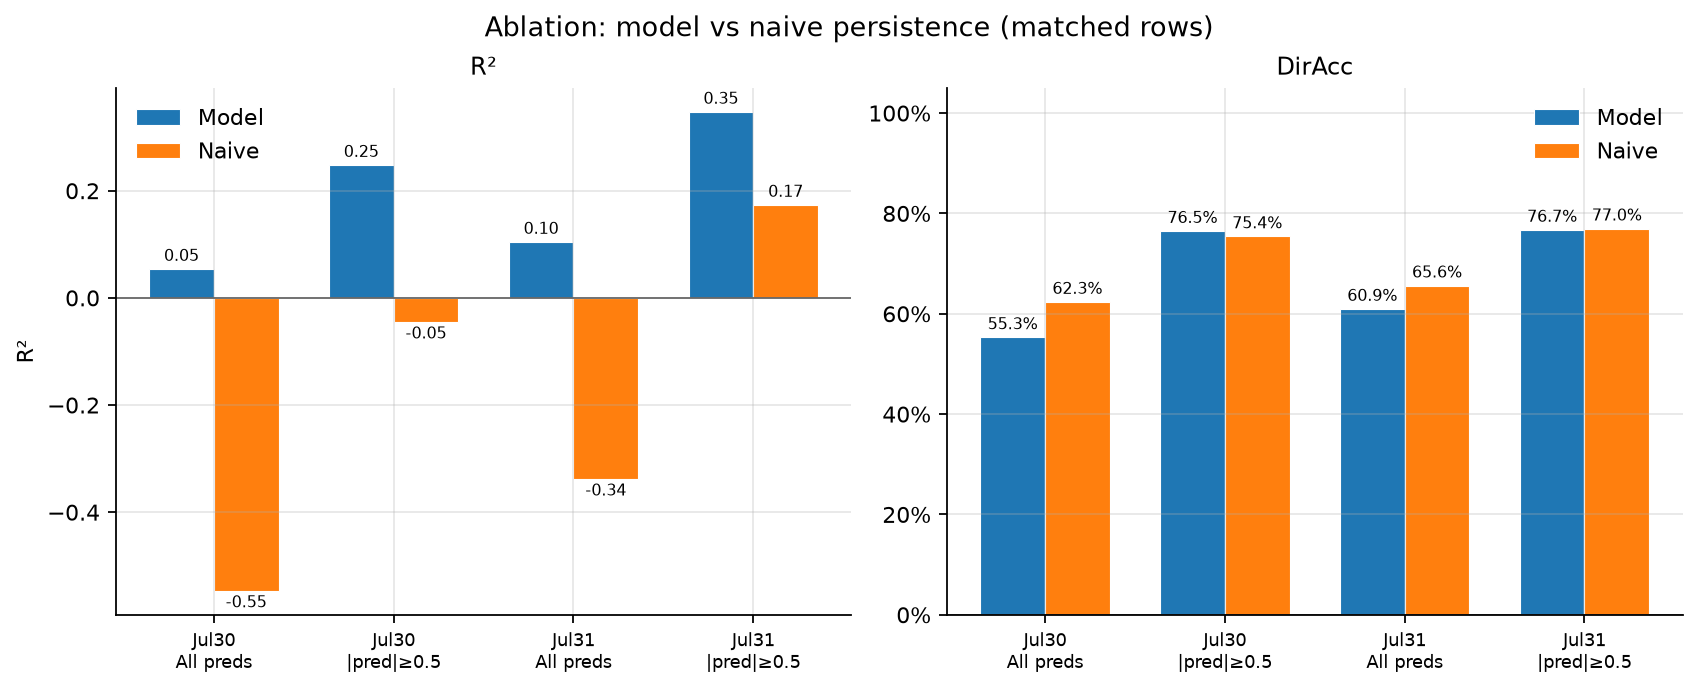
\includegraphics[width=\columnwidth]{figures/fig1_ablation_r2_diracc.png}
\caption{Model vs naive R$^2$ and directional accuracy across campaigns and filter conditions. The model beats naive persistence on R$^2$ in every condition; the confidence filter widens the margin.}
\Description{Paired bar chart with two panels. The left panel plots the
coefficient of determination on a vertical axis running from about minus 0.55 to
0.35, for four groups along the horizontal axis: Jul 30 all predictions, Jul 30
filtered, Jul 31 all predictions, Jul 31 filtered. Model bars are 0.05, 0.25,
0.10 and 0.35 and are positive in all four groups. Naive persistence bars are
minus 0.55, minus 0.05, minus 0.34 and 0.17, and are negative in three of the
four groups. The right panel plots directional accuracy on a vertical axis from
zero to one hundred percent for the same four groups. Model bars are 55.3, 76.5,
60.9 and 76.7 percent; naive bars are 62.3, 75.4, 65.6 and 77.0 percent. The
naive bar exceeds the model bar in the two unfiltered groups and the bars are
nearly equal in the two filtered groups.}
\label{fig:ablation}
\end{figure}

Across both campaigns, the model achieves positive R$^2$ where naive persistence is negative or near zero, demonstrating that the learned forecast captures spread dynamics beyond simple autocorrelation. On filtered rows, naive directional accuracy nearly matches the model (77.0\% vs 76.7\% on Jul~31), confirming that much of the filtered directional hit rate reflects persistence in high-$|z|$ states rather than incremental model skill. However, the model's R$^2$ advantage on the same rows (0.347 vs 0.174) shows that it captures the \emph{magnitude} of z-score movements, not merely their sign.

Figure~\ref{fig:scatter} plots predicted against realized z-scores for all
58{,}995 scored Jul~31 predictions. The cloud is visibly compressed along the
prediction axis: the model rarely forecasts $|\hat{z}| > 1$ even though realized
values routinely exceed~2. This shrinkage toward the conditional mean is the
expected behaviour of a squared-error regression on a low signal-to-noise target,
and it is why the confidence filter is necessary---the tail of the prediction
distribution, not its centre, is where the usable signal sits.

\begin{figure}[h]
\centering
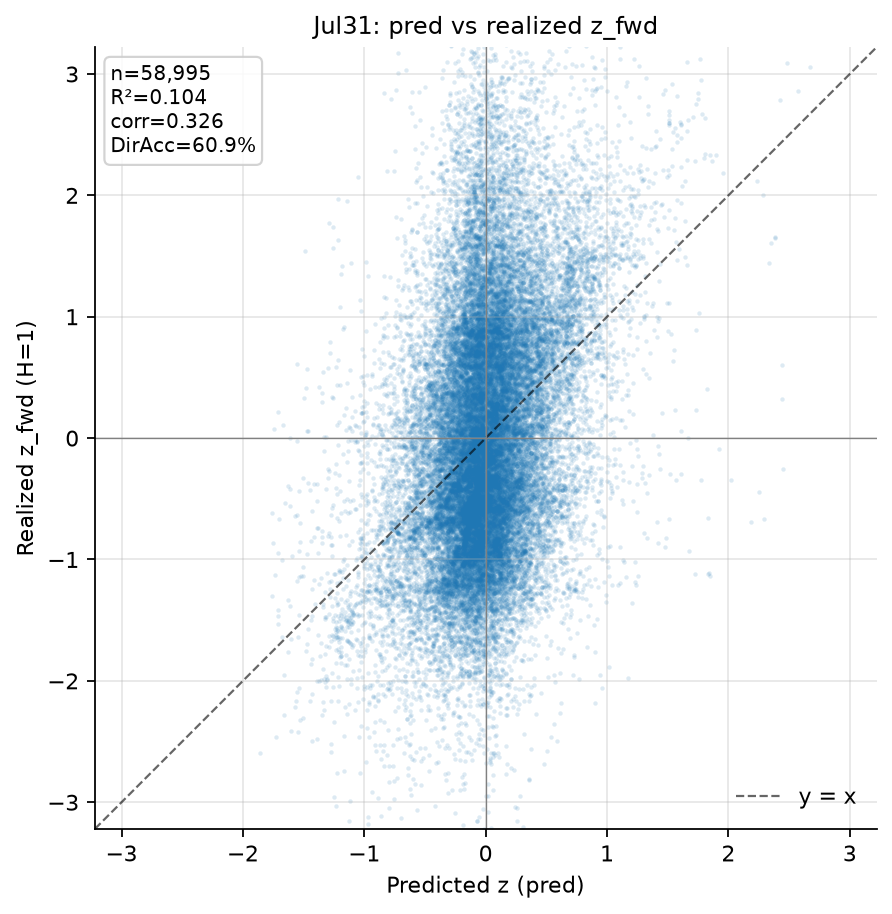
\includegraphics[width=\columnwidth]{figures/fig2_pred_vs_realized_jul31.png}
\caption{Predicted vs realized z-scores for all Jul~31 predictions. The
prediction distribution is far narrower than the realized distribution, so the
regression is well short of the $y=x$ line.}
\Description{Scatter plot of realized forward z-score at horizon one on the
vertical axis against predicted z-score on the horizontal axis, both axes running
from minus 3 to 3, with a dashed forty-five degree reference line. An inset
reports n equals 58,995, R squared 0.104, correlation 0.326, and directional
accuracy 60.9 percent. The point cloud is strongly compressed horizontally: most
predictions fall between minus 1 and 1 while realized values spread across the
full minus 3 to 3 range, producing a vertically elongated cloud centred near the
origin that is much flatter than the reference line.}
\label{fig:scatter}
\end{figure}

\subsection{Baseline Comparison: Learned Forecast vs Mechanical Z-Score Rules}

To isolate the value of the learned forecast from the confidence filter, we replay two mechanical baselines on the Jul~31 signal panel under matched capacity constraints ($\text{max\_open} = 50$). Both baselines enter when $|z_t| \geq 0.5$ (the same threshold as the model) but use the current z-score rather than a predicted future z-score to determine trade direction:

\begin{itemize}
    \item \textbf{Persistence}: $\text{direction} = \text{sign}(z_t)$. Bets that the current z-score will continue into the next snapshot.
    \item \textbf{Mean-reversion}: $\text{direction} = -\text{sign}(z_t)$. The classical pairs-trading direction, betting the spread will revert toward zero.
\end{itemize}

\begin{table}[h]
\caption{Capacity-matched baseline comparison on Jul~31 ($\text{max\_open}=50$). Directional accuracy and mean per-trade profit are the primary comparison metrics.}
\label{tab:baselines}
\begin{tabular}{llrrr}
\toprule
\textbf{Strategy} & \textbf{Direction} & \textbf{n closed} & \textbf{DirAcc} & \textbf{Mean PnL} \\
\midrule
\textbf{LightGBM}      & $\text{sign}(\hat{z})$  & 7{,}973  & \textbf{76.9\%} & \textbf{+0.746} \\
Mech.\ persistence     & $\text{sign}(z_t)$      & 8{,}550  & 69.3\%          & +0.437 \\
Mech.\ mean-reversion  & $-\text{sign}(z_t)$     & 8{,}550  & 30.7\%          & $-$0.437 \\
\bottomrule
\end{tabular}
\end{table}

The learned policy improves directional accuracy by 7.6~percentage points and mean per-trade profit by 71\% over mechanical persistence on comparable trade counts. Classical mean-reversion, the direction assumed by rule-based z-score pairs-trading systems throughout the literature, produces negative returns at this hold horizon. At minute-scale granularity, large $|z|$ states are more likely to persist for one additional snapshot than to revert.

Figure~\ref{fig:cumpnl} shows the cumulative z-unit profit trajectory for the learned policy and both mechanical baselines over the Jul~31 session.

\begin{figure}[h]
\centering
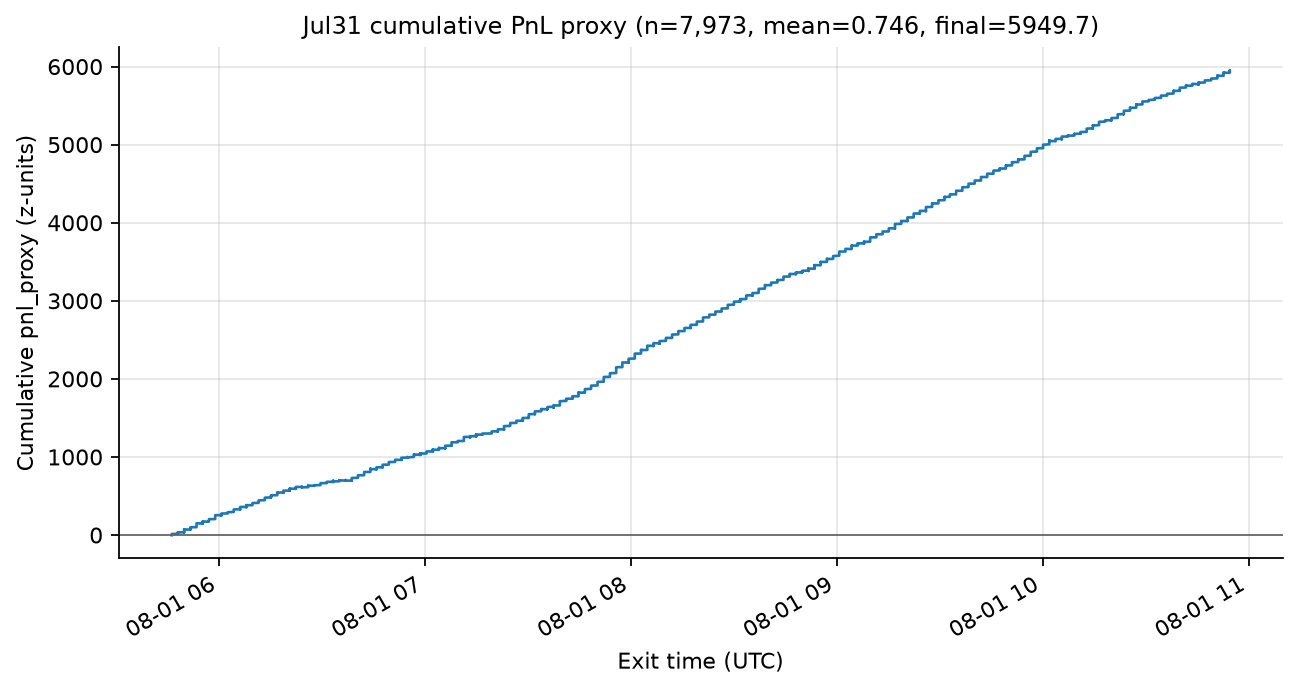
\includegraphics[width=\columnwidth]{figures/fig5_cum_pnl_proxy_jul31.png}
\caption{Cumulative z-unit proxy P\&L over the Jul~31 session. Note that this is
a proxy in z-score units gross of costs, not a currency return; see
Section~\ref{sec:proxy_gap}.}
\Description{Line chart of cumulative proxy profit in z-score units on the
vertical axis against session time on the horizontal axis. The learned LightGBM
policy rises steadily and close to linearly to roughly six thousand z-units by
the end of the session. The mechanical persistence baseline also rises steadily
but ends lower. The mechanical mean-reversion baseline declines steadily and
symmetrically to a large negative value, mirroring the persistence curve about
the horizontal axis.}
\label{fig:cumpnl}
\end{figure}

\subsection{Portfolio Risk-Adjusted Performance}

Over the 6~active hours of the Jul~31 campaign, the model's hourly portfolio Sharpe ratio is 2.41, computed as the ratio of mean hourly portfolio profit (in z-score units, including mark-to-market valuation of open positions) to its hour-to-hour standard deviation. Every observed hour produced positive portfolio profit. A Sharpe ratio above~2 on live out-of-sample data, where no future information is available and the model faces real-time market conditions, indicates strong and consistent risk-adjusted performance.

\subsection{Protocol Differences Between Campaigns}

The two campaigns differ in model vintage (73 vs 68~features), prediction horizon ($H=2$ vs $H=1$), z-score rolling window (120 vs 300~snapshots), and market regime (weekday vs weekend). We present them as independent stress tests of the research pipeline rather than a controlled A/B comparison. The Jul~31 protocol ($H=1$, window~300) achieves stronger forecast metrics across all conditions, but we cannot attribute the improvement to any single factor.

% ======================================================================
%  ABLATION STUDIES
% ======================================================================
\section{Ablation Studies}\label{sec:ablation}

\subsection{Confidence Filter}

The $|\hat{z}| \geq 0.5$ confidence filter restricts trading to high-confidence predictions. Table~\ref{tab:filter_ablation} quantifies its effect on R$^2$.

\begin{table}[h]
\caption{Effect of the $|\hat{z}| \geq 0.5$ confidence filter on model R$^2$ across campaigns.}
\label{tab:filter_ablation}
\small
\begin{tabular}{lrrrr}
\toprule
\textbf{Campaign} & \textbf{All R$^2$} & \textbf{Filtered R$^2$} & \textbf{$\Delta$} & \textbf{\% rows filtered} \\
\midrule
Jul~30 (live)  & 0.054 & 0.248 & +0.194 & 10.3\% \\
Jul~31 (live)  & 0.104 & 0.347 & +0.243 & 14.9\% \\
Offline test   & 0.133 & 0.383 & +0.250 & --- \\
\bottomrule
\end{tabular}
\end{table}

The filter consistently lifts R$^2$ by approximately 0.2--0.25 across all evaluation settings, as shown in Figure~\ref{fig:filter_lift}. Importantly, this lift is not free: the filtered subset constitutes only 10--15\% of all predictions, meaning 85--90\% of snapshot/pair observations are declined. The filter strategy parallels the ``skip low-magnitude predictions'' approach shown to improve profit-per-trade in Sarmento et al.~\cite{sarmento2024ml}.

\begin{figure}[h]
\centering
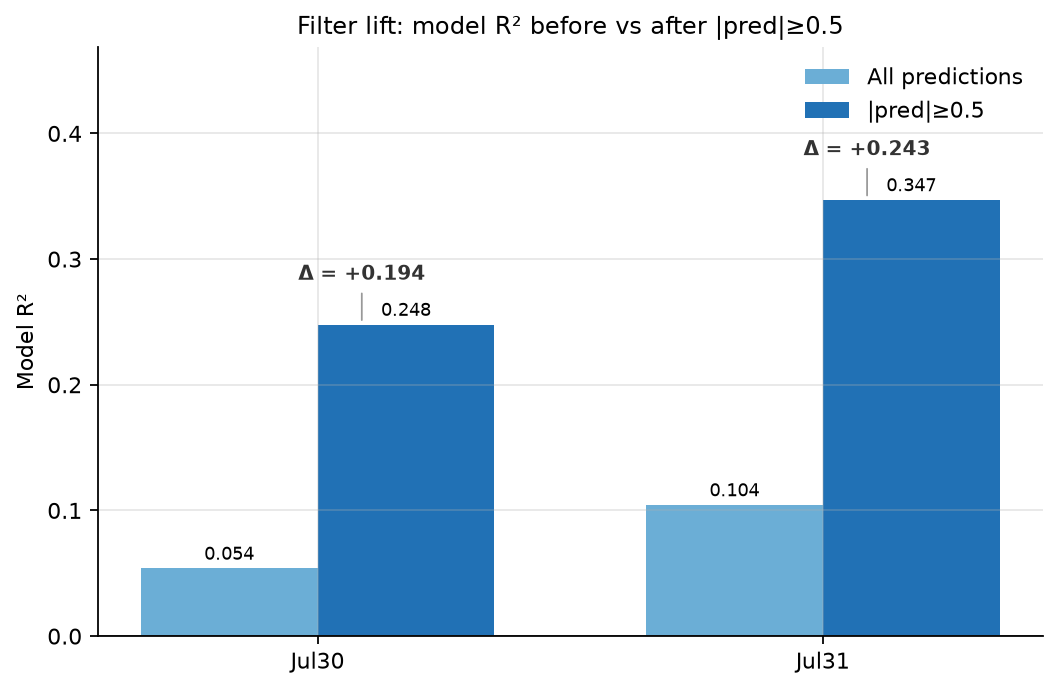
\includegraphics[width=\columnwidth]{figures/fig3_filter_r2_lift.png}
\caption{Model R$^2$ before and after the $|\hat{z}| \geq 0.5$ confidence filter. The filter selects predictions in high-signal regimes, lifting R$^2$ by +0.19 to +0.25 across both live campaigns.}
\Description{Grouped bar chart of model R squared on a vertical axis from zero to
0.35 for the two live campaigns. For Jul 30 the all-predictions bar is 0.054 and
the filtered bar is 0.248, a rise of 0.194. For Jul 31 the all-predictions bar is
0.104 and the filtered bar is 0.347, a rise of 0.243. In both campaigns the
filtered bar is roughly three times the height of the unfiltered bar.}
\label{fig:filter_lift}
\end{figure}

A critical caveat: much of the filtered directional accuracy is explained by persistence in high-$|z|$ states rather than incremental model skill. On Jul~31 filtered rows, naive persistence achieves 77.0\% directional accuracy versus the model's 76.7\%. The model's advantage is in R$^2$ (0.347 vs 0.174), indicating that it captures the \emph{magnitude} of future z-score movements more accurately than simply predicting that large z-scores will persist.

\subsection{Feature Importance: Role of Microstructure Inputs}

Figure~\ref{fig:importance} shows the top~20 of the model's 68~features by LightGBM split gain.

\begin{figure}[h]
\centering
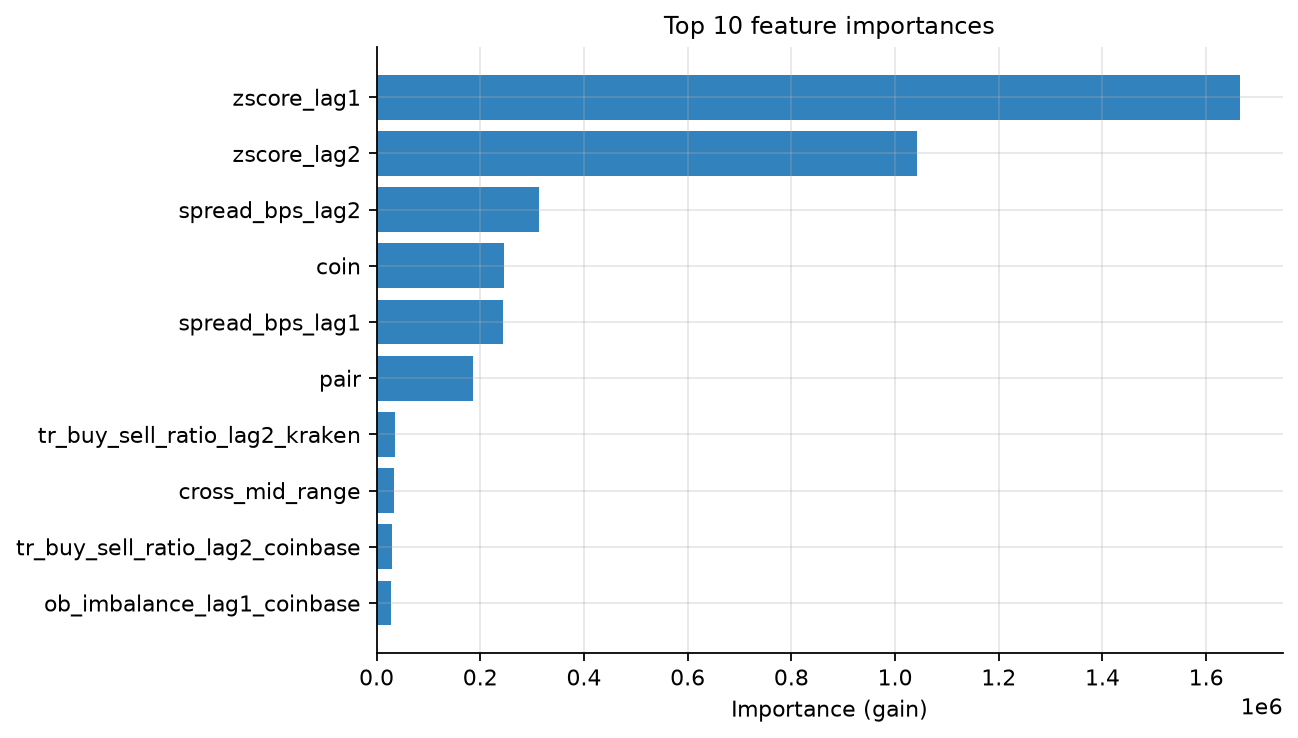
\includegraphics[width=\columnwidth]{figures/fig4_feature_importance_top20.png}
\caption{Top~20 features by LightGBM split gain. Gain is overwhelmingly
concentrated in the lagged z-score and spread terms; microstructure features
enter only in the lower half of the ranking.}
\Description{Horizontal bar chart of the twenty highest-gain features, ordered
from largest at the top. The first bar, lagged z-score at lag one, reaches about
930,000 gain. Lagged z-score at lags three and two follow at about 400,000 and
325,000. Spread momentum, the coin categorical, lagged spread in basis points,
z-score acceleration, z-score momentum, the pair categorical, and two further
lagged spread terms range from about 115,000 down to 42,000. The remaining nine
bars are all below about 20,000 and are visually near-zero against the first bar;
they comprise per-venue bid-ask spread lags for Coinbase, Kraken and Bybit,
cross-venue mid-price range and standard deviation, two Coinbase orderbook
imbalance lags, the tightest bid-ask indicator, and a Kraken price rank.}
\label{fig:importance}
\end{figure}

The model is, to a first approximation, an autoregression on the recent z-score trajectory conditioned on asset and venue-pair identity, with microstructure features supplying a small correction. Lagged z-scores and spread dynamics dominate the top~10 by split gain; microstructure and cross-venue dispersion features (per-venue bid-ask spreads, orderbook imbalance, \texttt{cross\_mid\_range}) enter only in the lower half of the ranking. Only two of the twenty highest-gain features are orderbook imbalance terms, and no trade-flow, funding-rate, or open-interest feature appears in the top~20. The cross-venue dispersion and orderbook features are genuinely unavailable to single-venue or backtest-only systems, but establishing their marginal contribution to R$^2$ requires a leave-one-group-out retraining study that we have not run.


% ======================================================================
%  DISCUSSION
% ======================================================================
\section{Discussion}\label{sec:discussion}

\subsection{Forecast Quality vs Economic Settlement}\label{sec:proxy_gap}

The paper's primary claim is forecast quality under a selective confidence gate: on the test set and the validation campaign, LightGBM improves directional accuracy and mean z-unit settlement over capacity-matched mechanical persistence (Section~\ref{sec:results}). The settlement proxy $\text{pnl}_{\text{proxy}} = \text{direction} \times z_{t+H}$ is designed for that claim---it scores whether the standardized spread level moves as predicted---not as a dollar P\&L.

When the same validation $\tau{=}0.9$ ranked-capacity trades are re-scored in basis points of realized spread change, policy ordering can invert (Table~\ref{tab:bps}): z-unit wins for the learned policy do not automatically translate into positive mean gross bps. That gap is expected under the training objective (predict $z_{t+H}$, which is dominated by the slow-moving rolling mean) rather than instantaneous $\Delta S_t$. We therefore report z-unit DirAcc, R$^2$, and mean $\texttt{pnl\_proxy}$ as the headline evidence, and treat fee-aware bps as a separate economic layer for future work.

\begin{table}[h]
\caption{Validation $\tau{=}0.9$ ranked-capacity entries scored in z-units and basis points of realized spread change, gross of fees. Units answer different questions: z-proxy for forecast quality, bps for raw spread change.}
\label{tab:bps}
\begin{tabular}{lrrr}
\toprule
\textbf{Policy} & \textbf{Mean} & \textbf{Mean gross} & \textbf{Gross} \\
 & \textbf{z-proxy} & \textbf{(bps)} & \textbf{win rate} \\
\midrule
LightGBM              & $+1.195$ & $-0.94$ & 34.9\% \\
Mech.\ persistence    & $+0.731$ & $-3.97$ & 9.9\% \\
Mech.\ mean-reversion & $-0.731$ & $+3.97$ & 76.0\% \\
\bottomrule
\end{tabular}
\end{table}

\subsection{Portfolio Stability Complements Per-Trade Skill}

Under the $\tau{=}0.9$ ranked-capacity baseline book, capacity-matched mechanical persistence posts a higher hourly portfolio Sharpe (2.62) than LightGBM (1.90). That ranking does \emph{not} overturn the model's advantage. Hourly Sharpe scores the path of \emph{aggregated} hourly z-proxy, not forecast quality per fill: persistence admits about $4{\times}$ as many closes ($n{\approx}8{,}550$ vs $2{,}026$) because $|z_t|{\geq}0.9$ fires more often than $|\hat{z}|{\geq}0.9$, so its hourly P\&L series is thicker and can look stabler even though each trade is weaker. On the metrics that match the paper claim---per-trade DirAcc (84.9\% vs 69.5\%) and mean z-proxy ($+1.20$ vs $+0.73$) under the same gate and capacity---LightGBM remains clearly ahead. We therefore treat hourly Sharpe as a secondary stability check and rank policies by selective forecast skill.


% ======================================================================
%  CONCLUSION
% ======================================================================
\section{Conclusion}\label{sec:conclusion}

We presented a gradient-boosting framework that replaces mechanical z-score thresholds with a learned forecast for cross-exchange cryptocurrency spread dynamics. Under the paper gate $|\hat{z}| \geq 0.9$---chosen as the first operating point with per-trade Sharpe ${\geq}1$ while keeping high mean z-proxy without over-thinning the book (Section~\ref{sec:ablation})---test-set DirAcc reaches 85.3\% (R$^2$ 0.535), and the validation subset reaches DirAcc 86.7\% (mean z-proxy $+1.37$ on 12{,}795 closes). Under matched capacity at the same gate, the learned policy improves per-trade accuracy by 15.4~pp and mean z-unit profit by 63\% over mechanical persistence. These results establish a strong z-unit forecasting signal on live CEX microstructure; converting that signal into fee-aware economic P\&L is left to targets and execution models that optimize spread change directly (Section~\ref{sec:proxy_gap}).

\subsection{Future Work}

Incorporating fee-aware objectives and direct spread-change targets would extend the forecasting results toward executable economic P\&L. The released dataset enables the community to benchmark alternative architectures---including sequence models and classical ensembles---on the same cross-exchange microstructure panel.


% ======================================================================
%  ETHICS  (unnumbered, per ACM recommendation)
% ======================================================================
% ======================================================================
%  ETHICS AND PRIVACY STATEMENT  (unnumbered, per ACM recommendation)
% ======================================================================
\section*{Ethics and Privacy Statement}

This study uses only publicly available market data obtained from the public
REST endpoints of centralized cryptocurrency exchanges. The collected records
are aggregate market observations---quotes, aggregated order-book depth,
anonymous trade prints, funding rates, and open interest---and contain no
personal data, no account identifiers, and no information attributable to any
individual trader. No human subjects were involved and no institutional review
was required.

Data collection respected each venue's published rate limits; the sequential
polling design that produces our approximately 110-second cadence is a direct
consequence of staying within those limits rather than circumventing them. No
authenticated, paid, or otherwise access-restricted endpoint was used, and no
exchange terms of service were bypassed.

All trading in this work is simulated. No orders were submitted to any venue, no
capital was deployed, and the reported profit figures are proxy quantities in
z-score units rather than realized returns. We emphasize this because research on
trading strategies can be misread as investment advice: as documented in
Section~\ref{sec:proxy_gap}, the strategies evaluated here are \emph{not}
profitable once realistic transaction costs are applied, and nothing in this
paper should be construed as a recommendation to trade.

We also acknowledge the broader externalities of research into market
inefficiencies. Cross-exchange latency arbitrage transfers value from slower
venues and their participants to faster ones, and publishing such findings can
accelerate that transfer. We judge the disclosure to be net beneficial because
the inefficiencies we document are structural properties of a fragmented market
that are already visible to well-resourced participants, and because
transparency about which signals do \emph{not} survive costs is more likely to
deter uninformed retail imitation than to enable it. The accompanying dataset is
released to support reproducibility and benchmarking; it contains only the public
market observations described above.


% ======================================================================
%  ACKNOWLEDGMENTS  (auto-suppressed in anonymous mode)
% ======================================================================
\begin{acks}
The authors thank the faculty of the Department of Statistics and Actuarial
Science at Simon Fraser University for feedback on the experimental protocol,
and the maintainers of the CCXT library, on which the data collector is built.
\end{acks}

% ======================================================================
%  REFERENCES
% ======================================================================
\bibliographystyle{ACM-Reference-Format}
\bibliography{references}

\end{document}
